\documentclass{beamer}
\usetheme[numbering=fraction, progressbar=frametitle]{metropolis}
\setbeamercovered{transparent}
\usepackage{pgfpages}
\setbeameroption{show notes on second screen=right}

\usepackage[utf8]{inputenc}
\usepackage[T1]{fontenc}
\usepackage{lmodern}
\usepackage[ngerman]{babel}
\usepackage{datetime}

\title{Zukunft der Raumfahrt}
\date{\today}
\author{Jens Juhl, Torben Mehner}
\institute{KIT}
\begin{document}
\maketitle

\begin{frame}{Inhaltsverzeichnis}
	\tableofcontents[sectionstyle=show,subsectionstyle=show]
\end{frame}

\section{Nahe Zukunft}
\subsection{NASA - Journey to Mars}
\begin{frame}{\insertsection: \insertsubsection}
	\begin{minipage}{.45\textwidth}
		Heute - Mitte 2020: \\
		\textbf{Earth Reliant} \\
		\note<1>{Earth Reliant
			\begin{itemize}
				\item ISS bis 2024
				\item Kommerzielle Raumfahrt im erdnahen Orbit
				\item Entwicklung von Systemen für interplanetare Raumfahrt
			\end{itemize}}
		
		\pause
		
		2018 - 2030: \\
		\textbf{Proving Ground} \\
		\note<2>{
			Proving Ground
			\begin{itemize}
				\item Regelmäßige, bemannte Missionen im Mondorbit
				\item Durch jahrelange Missionen beweisen, dass Habitate im 
				weiten All funktionieren
				\item Einfangen eines Asteroids und Platzierung im Mond-Orbit. 
				Dann sollen Astronuten robotergestützt Proben nehmen.
			\end{itemize}
			}
		\pause
		
		Heute - 2030 und länger: \\
		\textbf{Earth Independant}
		\note<3>{
			Earth Independant
			\begin{itemize}
				\item Missionen erforschen Mars
				\item Demonstration von Eintritt, Landung und 
				In-Situ-Ressourcenverwendung
				\item Unbemannte Missionen mit Rückkehr zum Mars
				\item In den frühen 2030ern: Menschen sollen den Mars umrunden
			\end{itemize}
		}
		
	\end{minipage} \quad
	\begin{minipage}{.5\textwidth}
		\only<1>{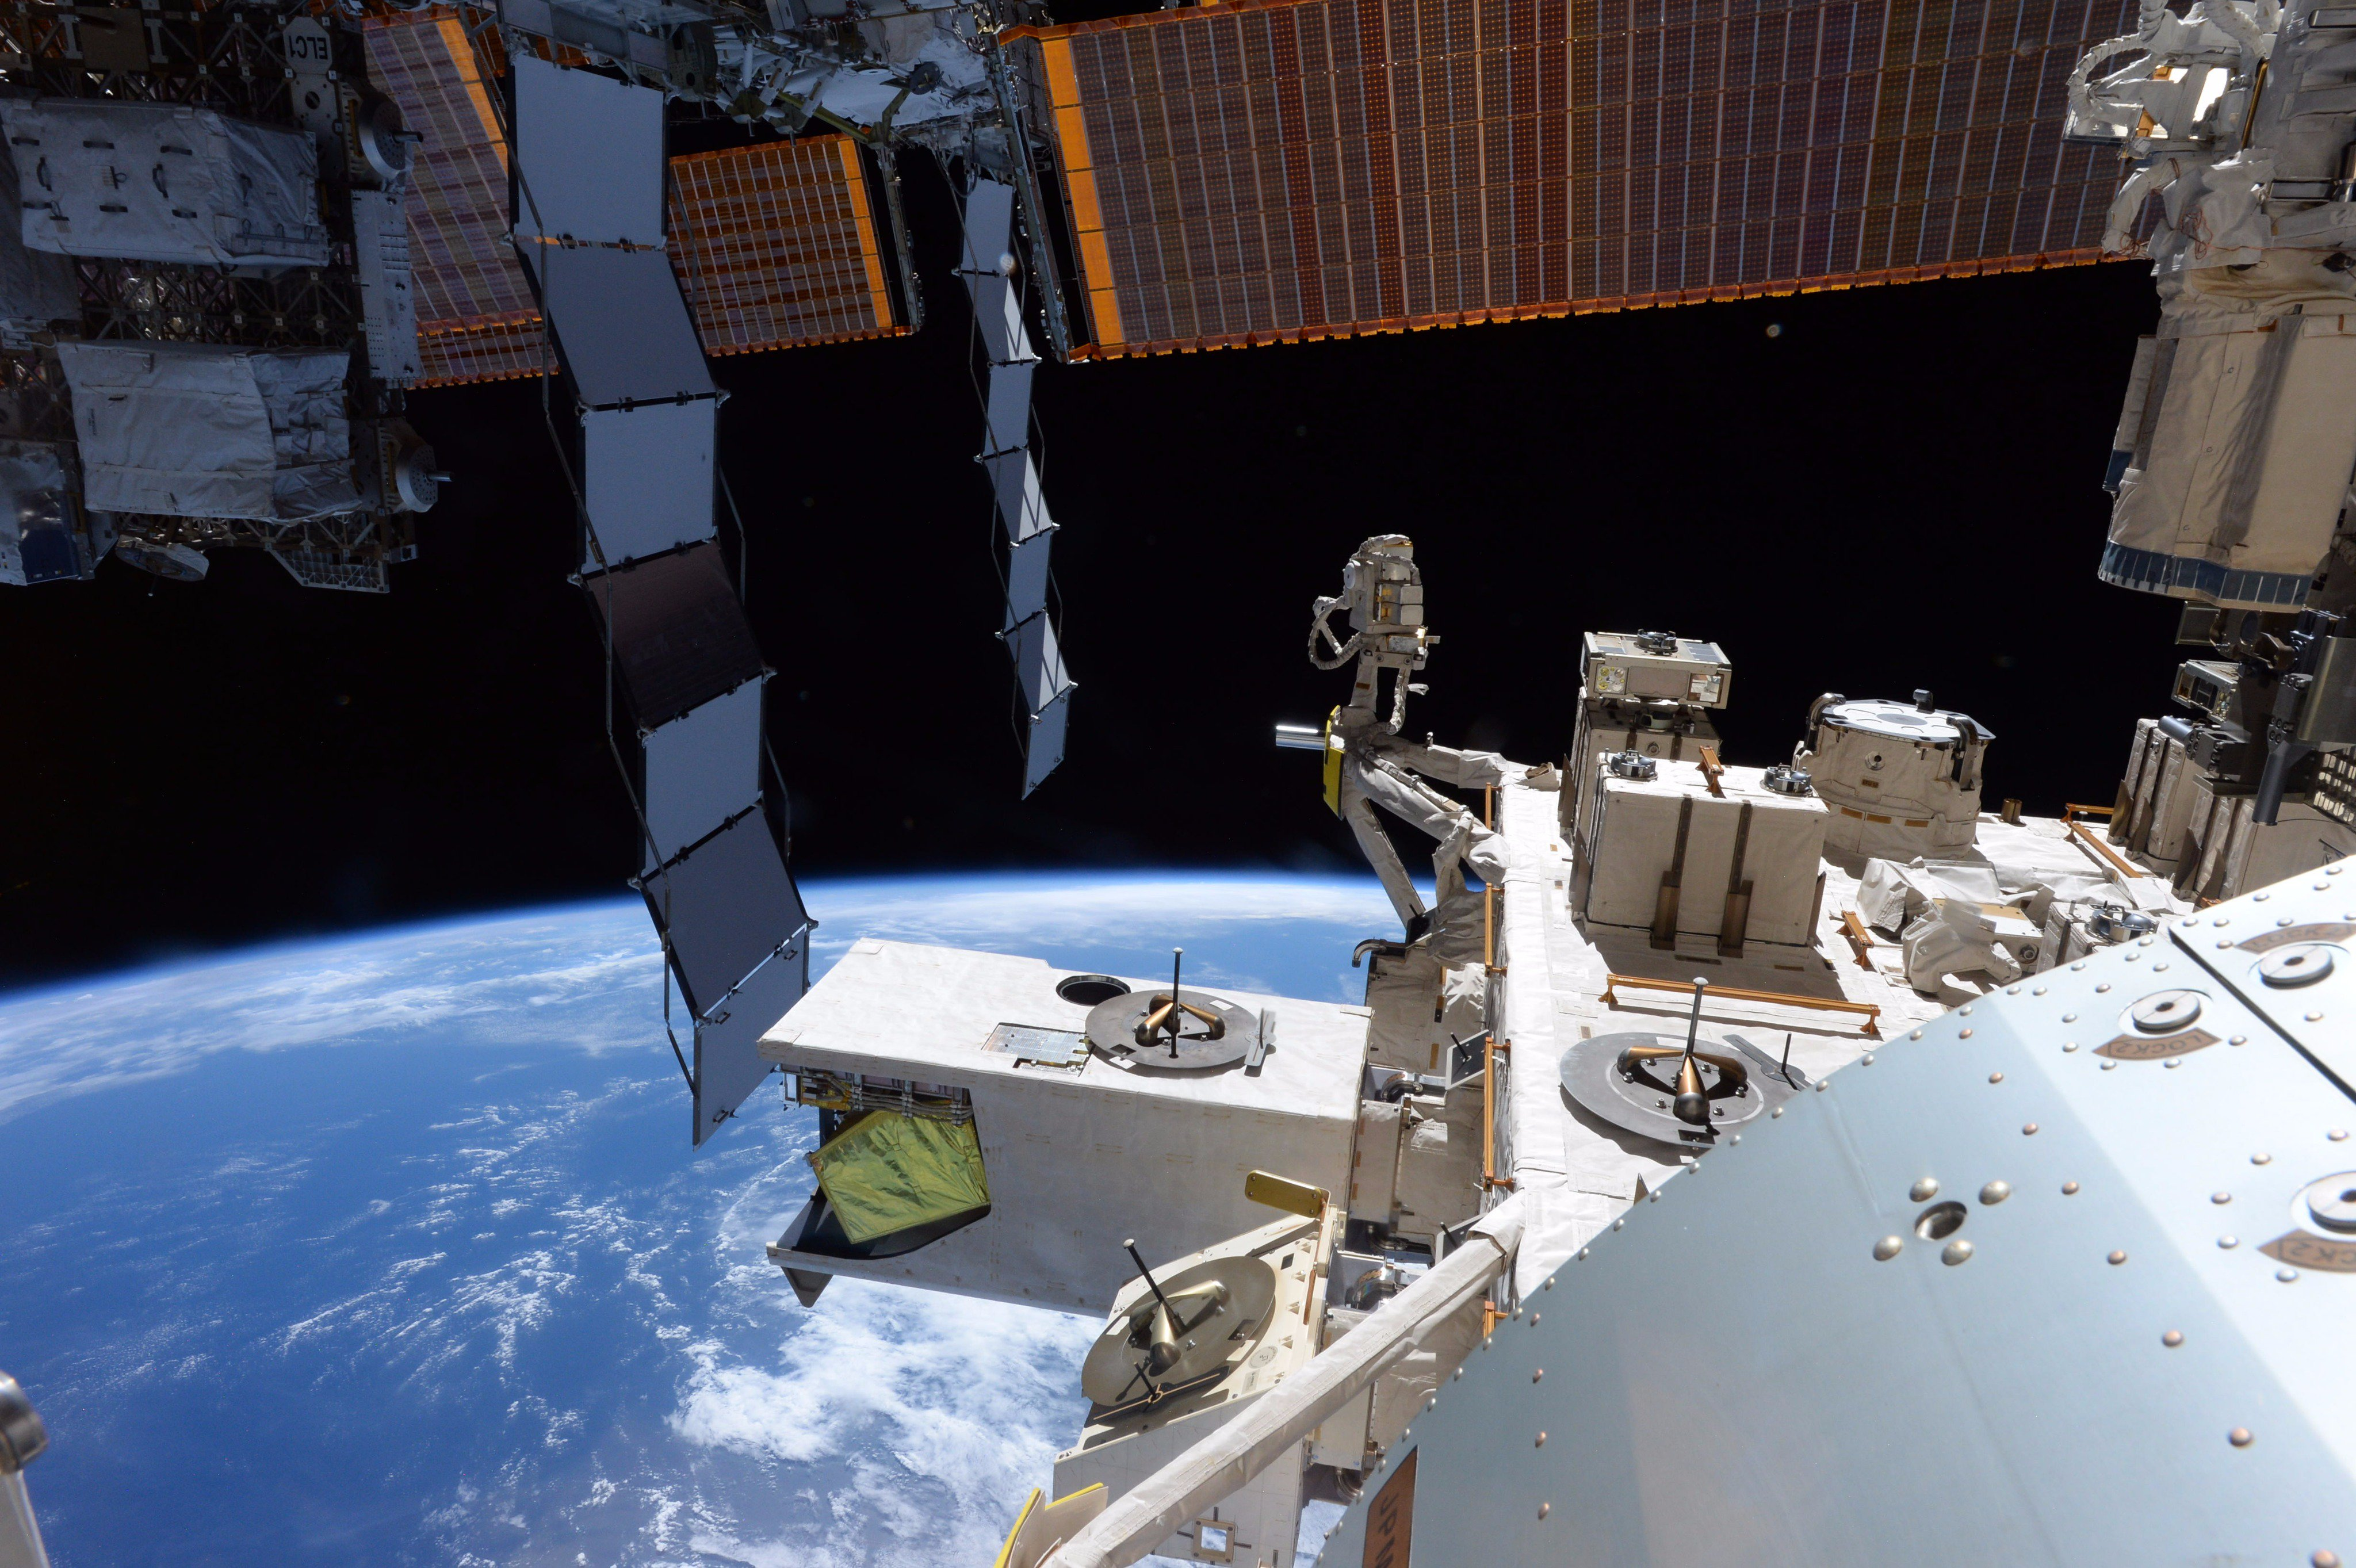
\includegraphics[width=\linewidth]{iss}
		
		{\tiny An Astronaut's View From the 'Corner Office',
		\\ Quelle: nasa.gov}}
		\only<2>{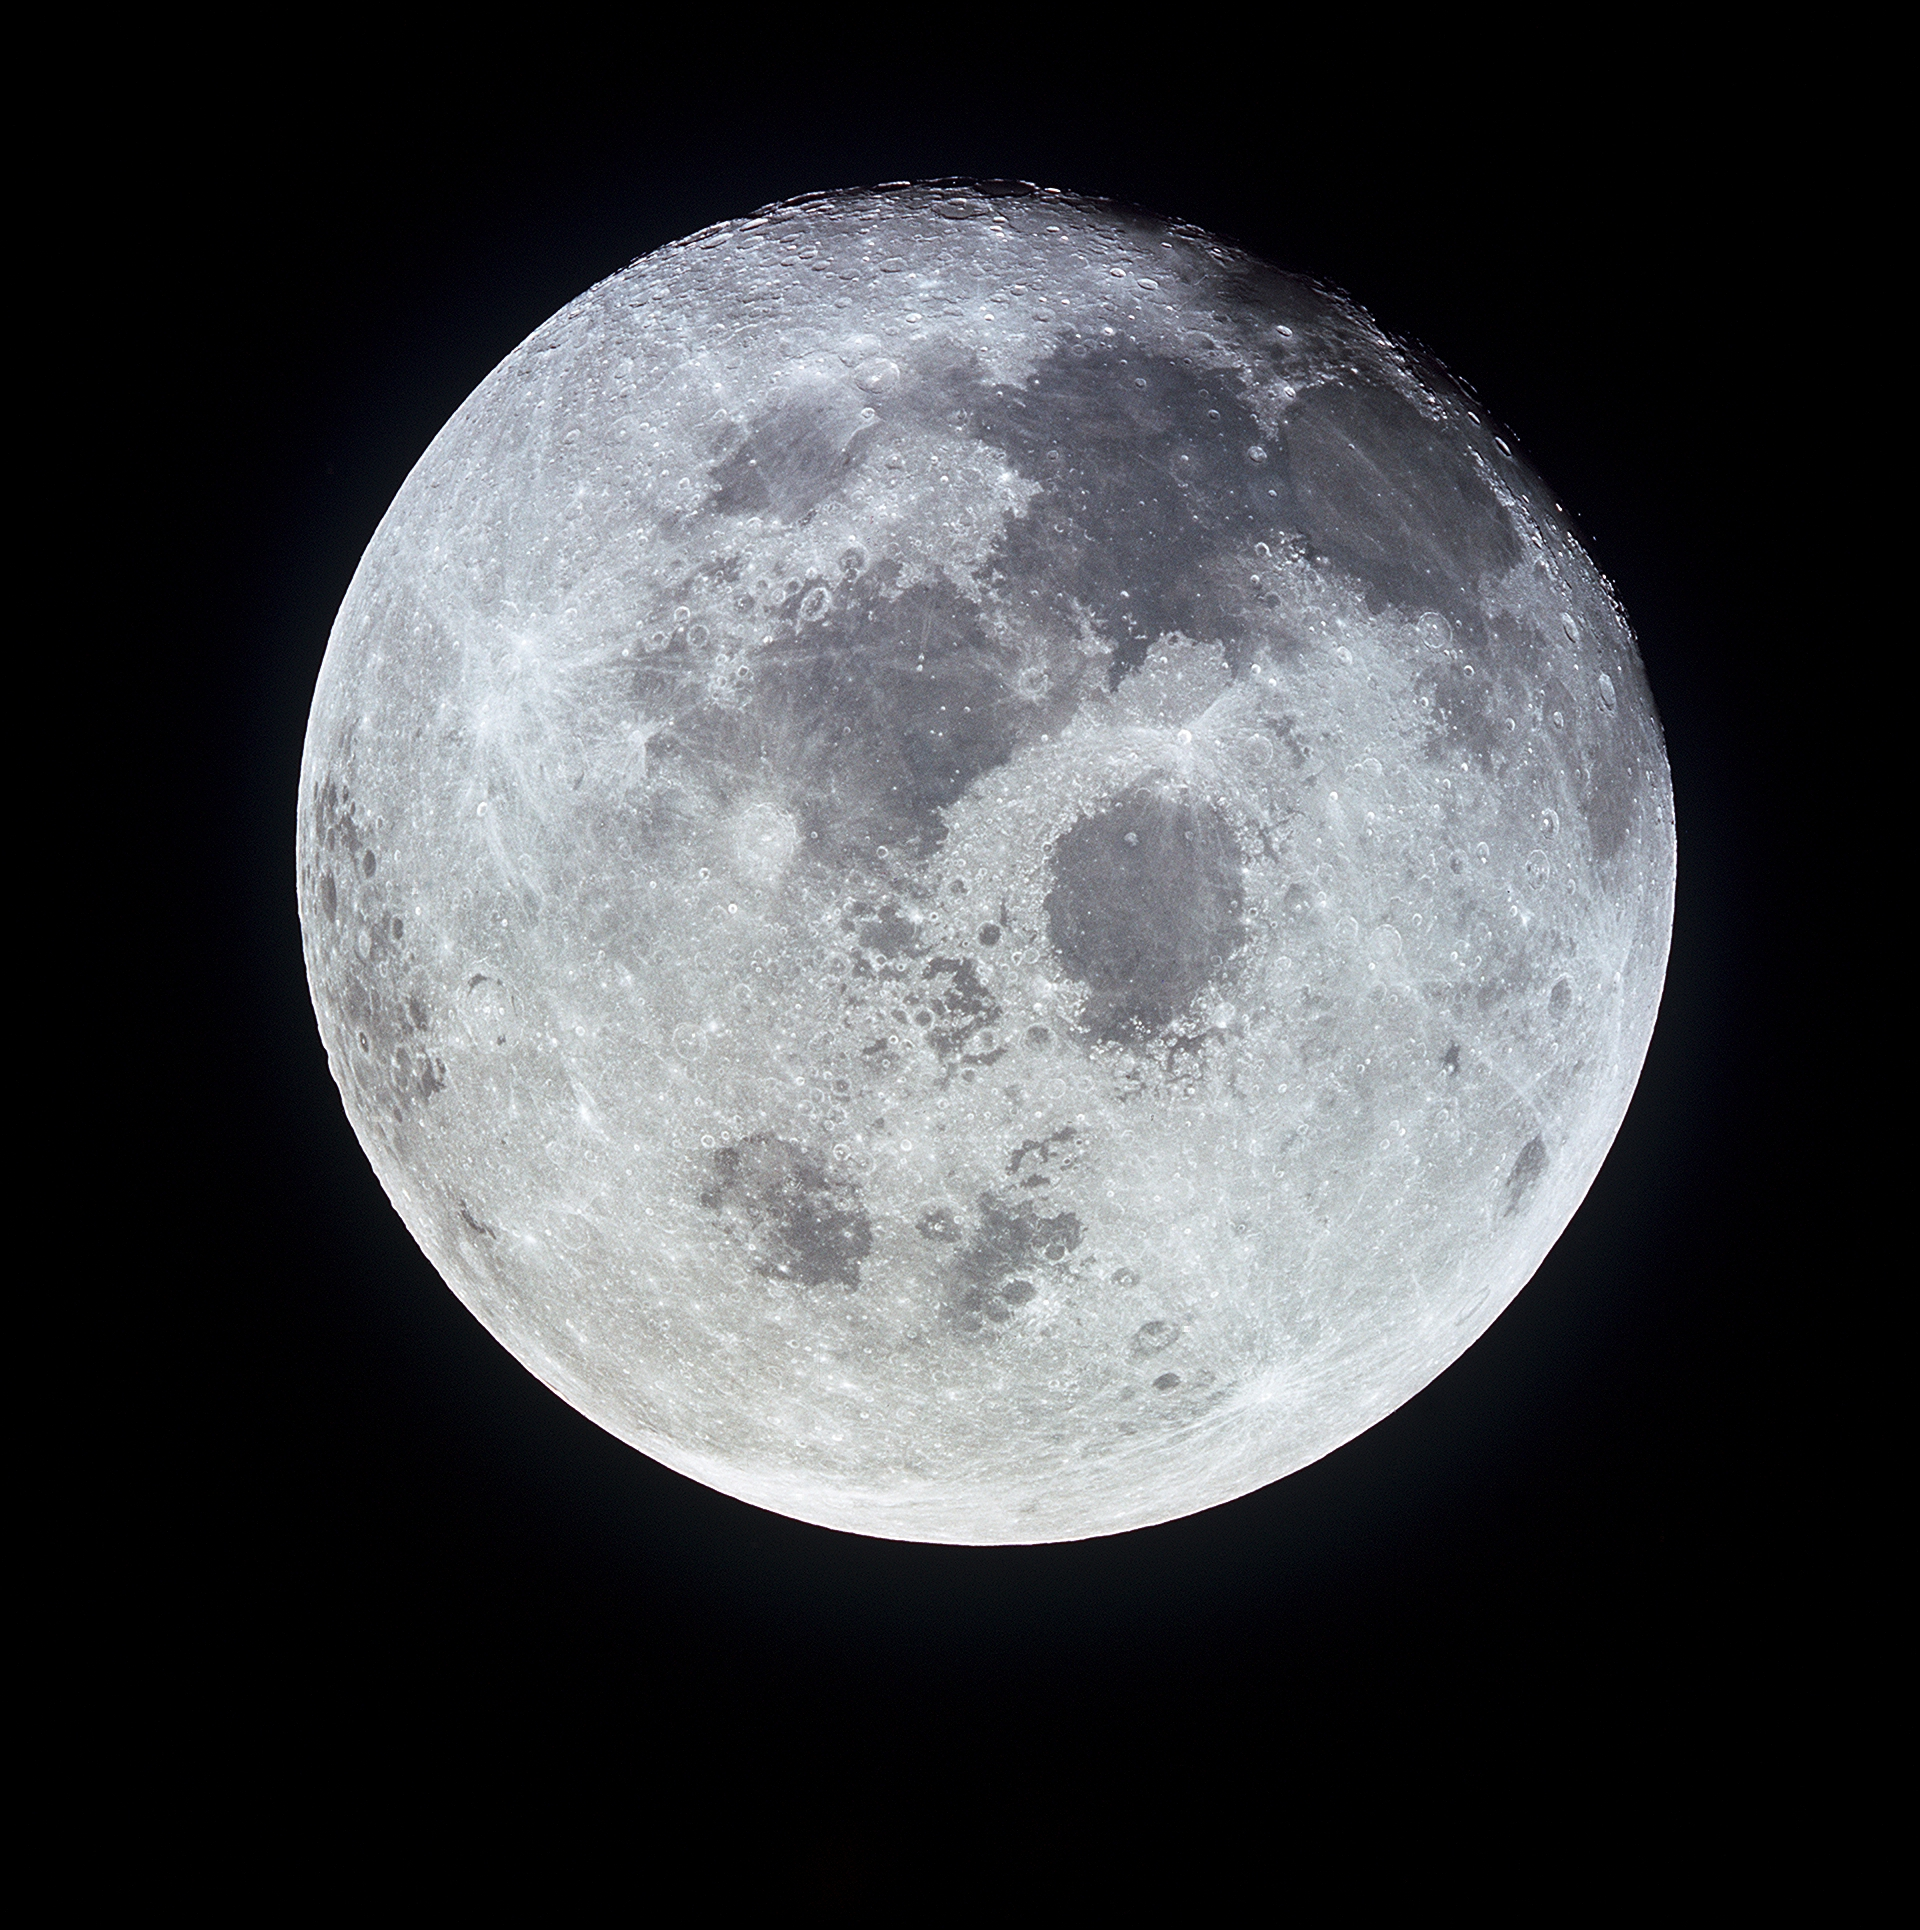
\includegraphics[width=\linewidth]{moon}
			
		{\tiny Photo of full Moon taken at Apollo 11 mission,
		\\ Quelle: nasa.gov}}

		\only<3>{\includegraphics[width=\linewidth]{mars}
			
		{\tiny Curiosity Self-Portrait at 'Murray Buttes',
		\\ Quelle: nasa.gov}}
	\end{minipage}
\end{frame}

\subsection{ESA und Roscosmos - ExoMars}
\begin{frame}{\insertsection: \insertsubsection}
	\begin{minipage}{.45\textwidth}
		
		Heute - 2024: \\
		\textbf{ISS} \\
		 \note<1>{
			 ISS:
			 \begin{itemize}
			 	\item Deutschland hat die finanziellen Mittel bereitgestellt
			 \end{itemize}
		 }
		
		\pause
		
		2016 - 2022: \\
		\textbf{TGO und Schiaparelli} \\
		\note<2>{Schiaparelli
			\begin{itemize}
				\item TGO: Trace Gas Orbiter
				\item Nachweis von Stoffwechselprodukten
				\item Schiaparelli bei Landung (Oktober 2016) zerschellt
			\end{itemize}}
		
		\pause
		
		Ab 2020: \\
		\textbf{ExoMars Rover} \\
		\note<3>{ExoMars Rover
			\begin{itemize}
				\item Sucht Leben auf dem Mars
				\item Hat einen Bohrer um tiefe Schichten zu erreichen (2m 
				Maximum)
				\item Hat viele Analyseinstrumente um Zusammensetzung des 
				Bodens zu bestimmen
				\item Fährt autonom bis zu 100m pro Sol (Mars-Tag). Verbindung 
				zur ESA nur ein bis zwei mal pro Sol möglich.
			\end{itemize}}
				
		\end{minipage} \quad
		\begin{minipage}{.5\textwidth}
			\only<1>{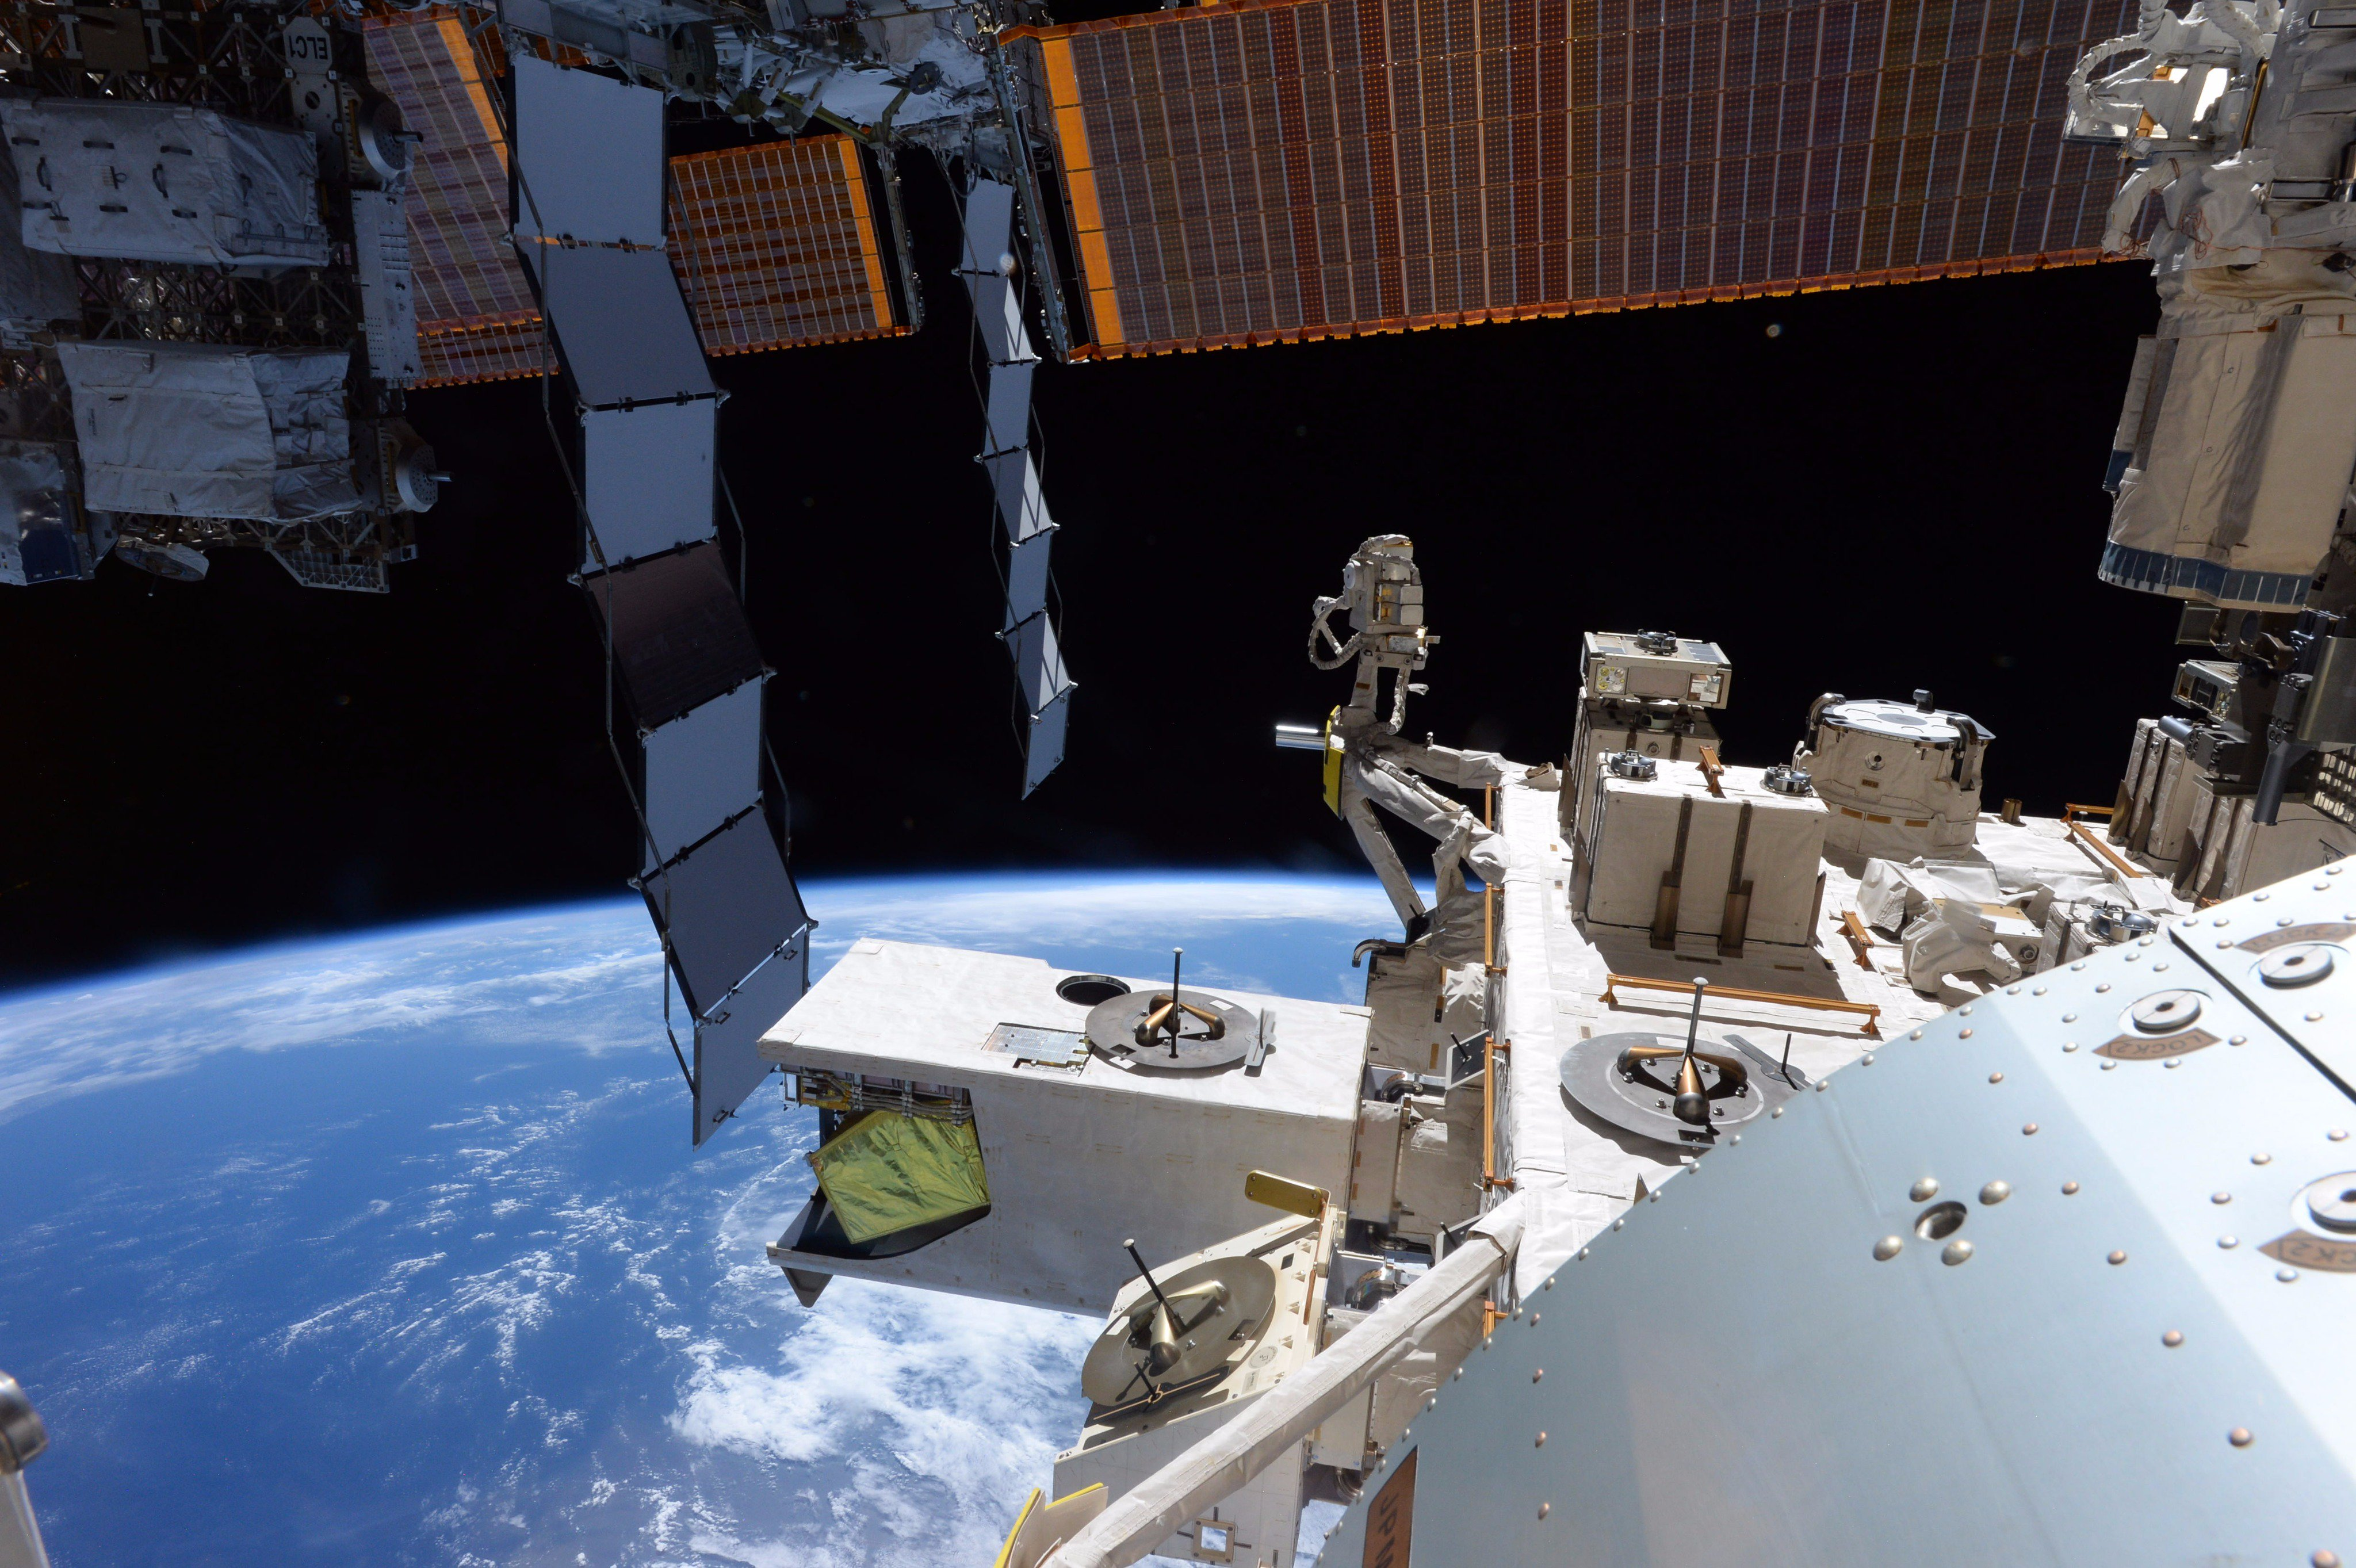
\includegraphics[width=\linewidth]{iss}
				
				{\tiny An Astronaut's View From the 'Corner Office',
					\\ Quelle: nasa.gov}}
			\only<2>{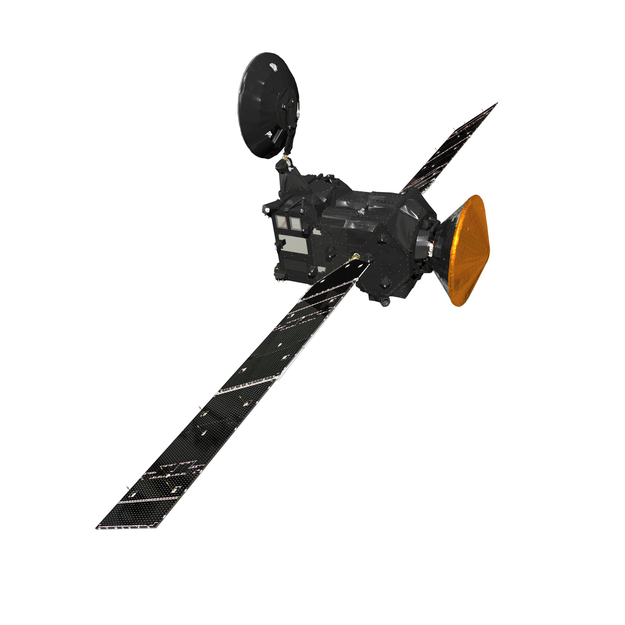
\includegraphics[width=\linewidth]{schiaparelli}
				
				{\tiny ExoMars 2016: Trace Gas Orbiter and Schiaparelli,
					\\ Quelle: esa.int}}
			\only<3>{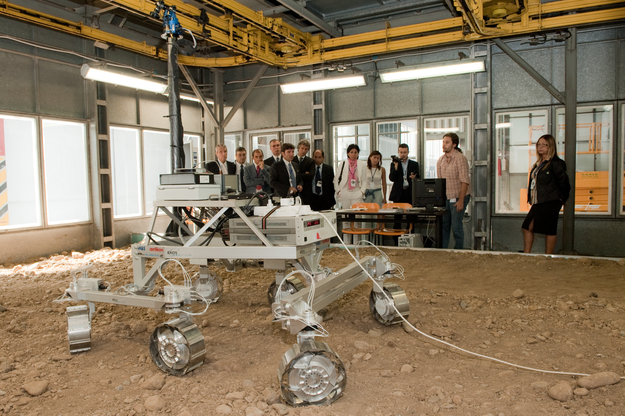
\includegraphics[width=\linewidth]{exomars}
				
				{\tiny The ExoMars Rover Prototype,
					\\ Quelle: esa.int}}
		\end{minipage}
	\end{frame}
	
\subsection{ESA - Kommerziell}
\begin{frame}{\insertsection: \insertsubsection}
	\begin{minipage}{.45\textwidth}
		
		Heute - 2020: \\
		\textbf{Umrüsung auf Ariane VI} \\
		
		\note{
			\begin{itemize}
				\item Preis pro kg bei 11to: 8000 Euro (4 Booster)
				\item Preis pro kg bei 4,5to: 16700 Euro (2Booster)
				\item Falcon 9 pro kg bei 8,5to: 7500 Euro
				\item Falcon Heavy pro kg bei 26,7to: 3400 Euro
			\end{itemize}
			}
				
			\end{minipage} \quad
			\begin{minipage}{.5\textwidth}
				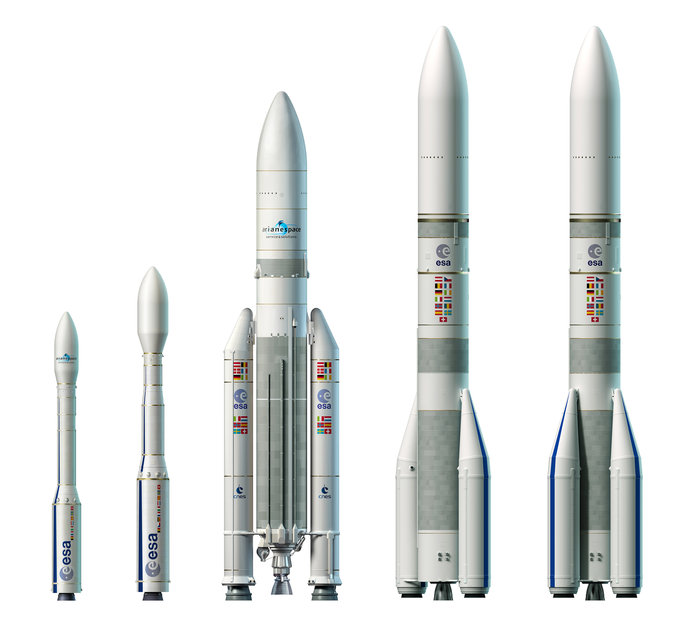
\includegraphics[width=\linewidth]{arianevi}
					
					{\tiny Artist's view of Vega, Vega-C, Ariane 5 ECA and the 
					two configurations of Ariane 6,
						\\ Quelle: esa.int}
			\end{minipage}
\end{frame}

\subsection{SpaceX}
\begin{frame}{\insertsection: \insertsubsection}
	\begin{minipage}{.45\textwidth}
		
		Ab 2022: \\
		\textbf{Making Life Multiplanetary} \\
		
		\note<1>{
			\begin{itemize}
				\item 2022: unbemannte Versorgungsmission
				\item 2024: erste bemannte Mission
			\end{itemize}
		}
		
		\pause
		
		Ab 2022: \\
		\textbf{BFR | Earth to Earth} \\
		
		\note<2>{
			\begin{itemize}
				\item BFR: Rakete der Marsmission
				\item Slogan: Um die halbe Welt in weniger als 30 Minuten
			\end{itemize}
		}
		
		
	\end{minipage} \quad
	\begin{minipage}{.5\textwidth}	
		\only<1>{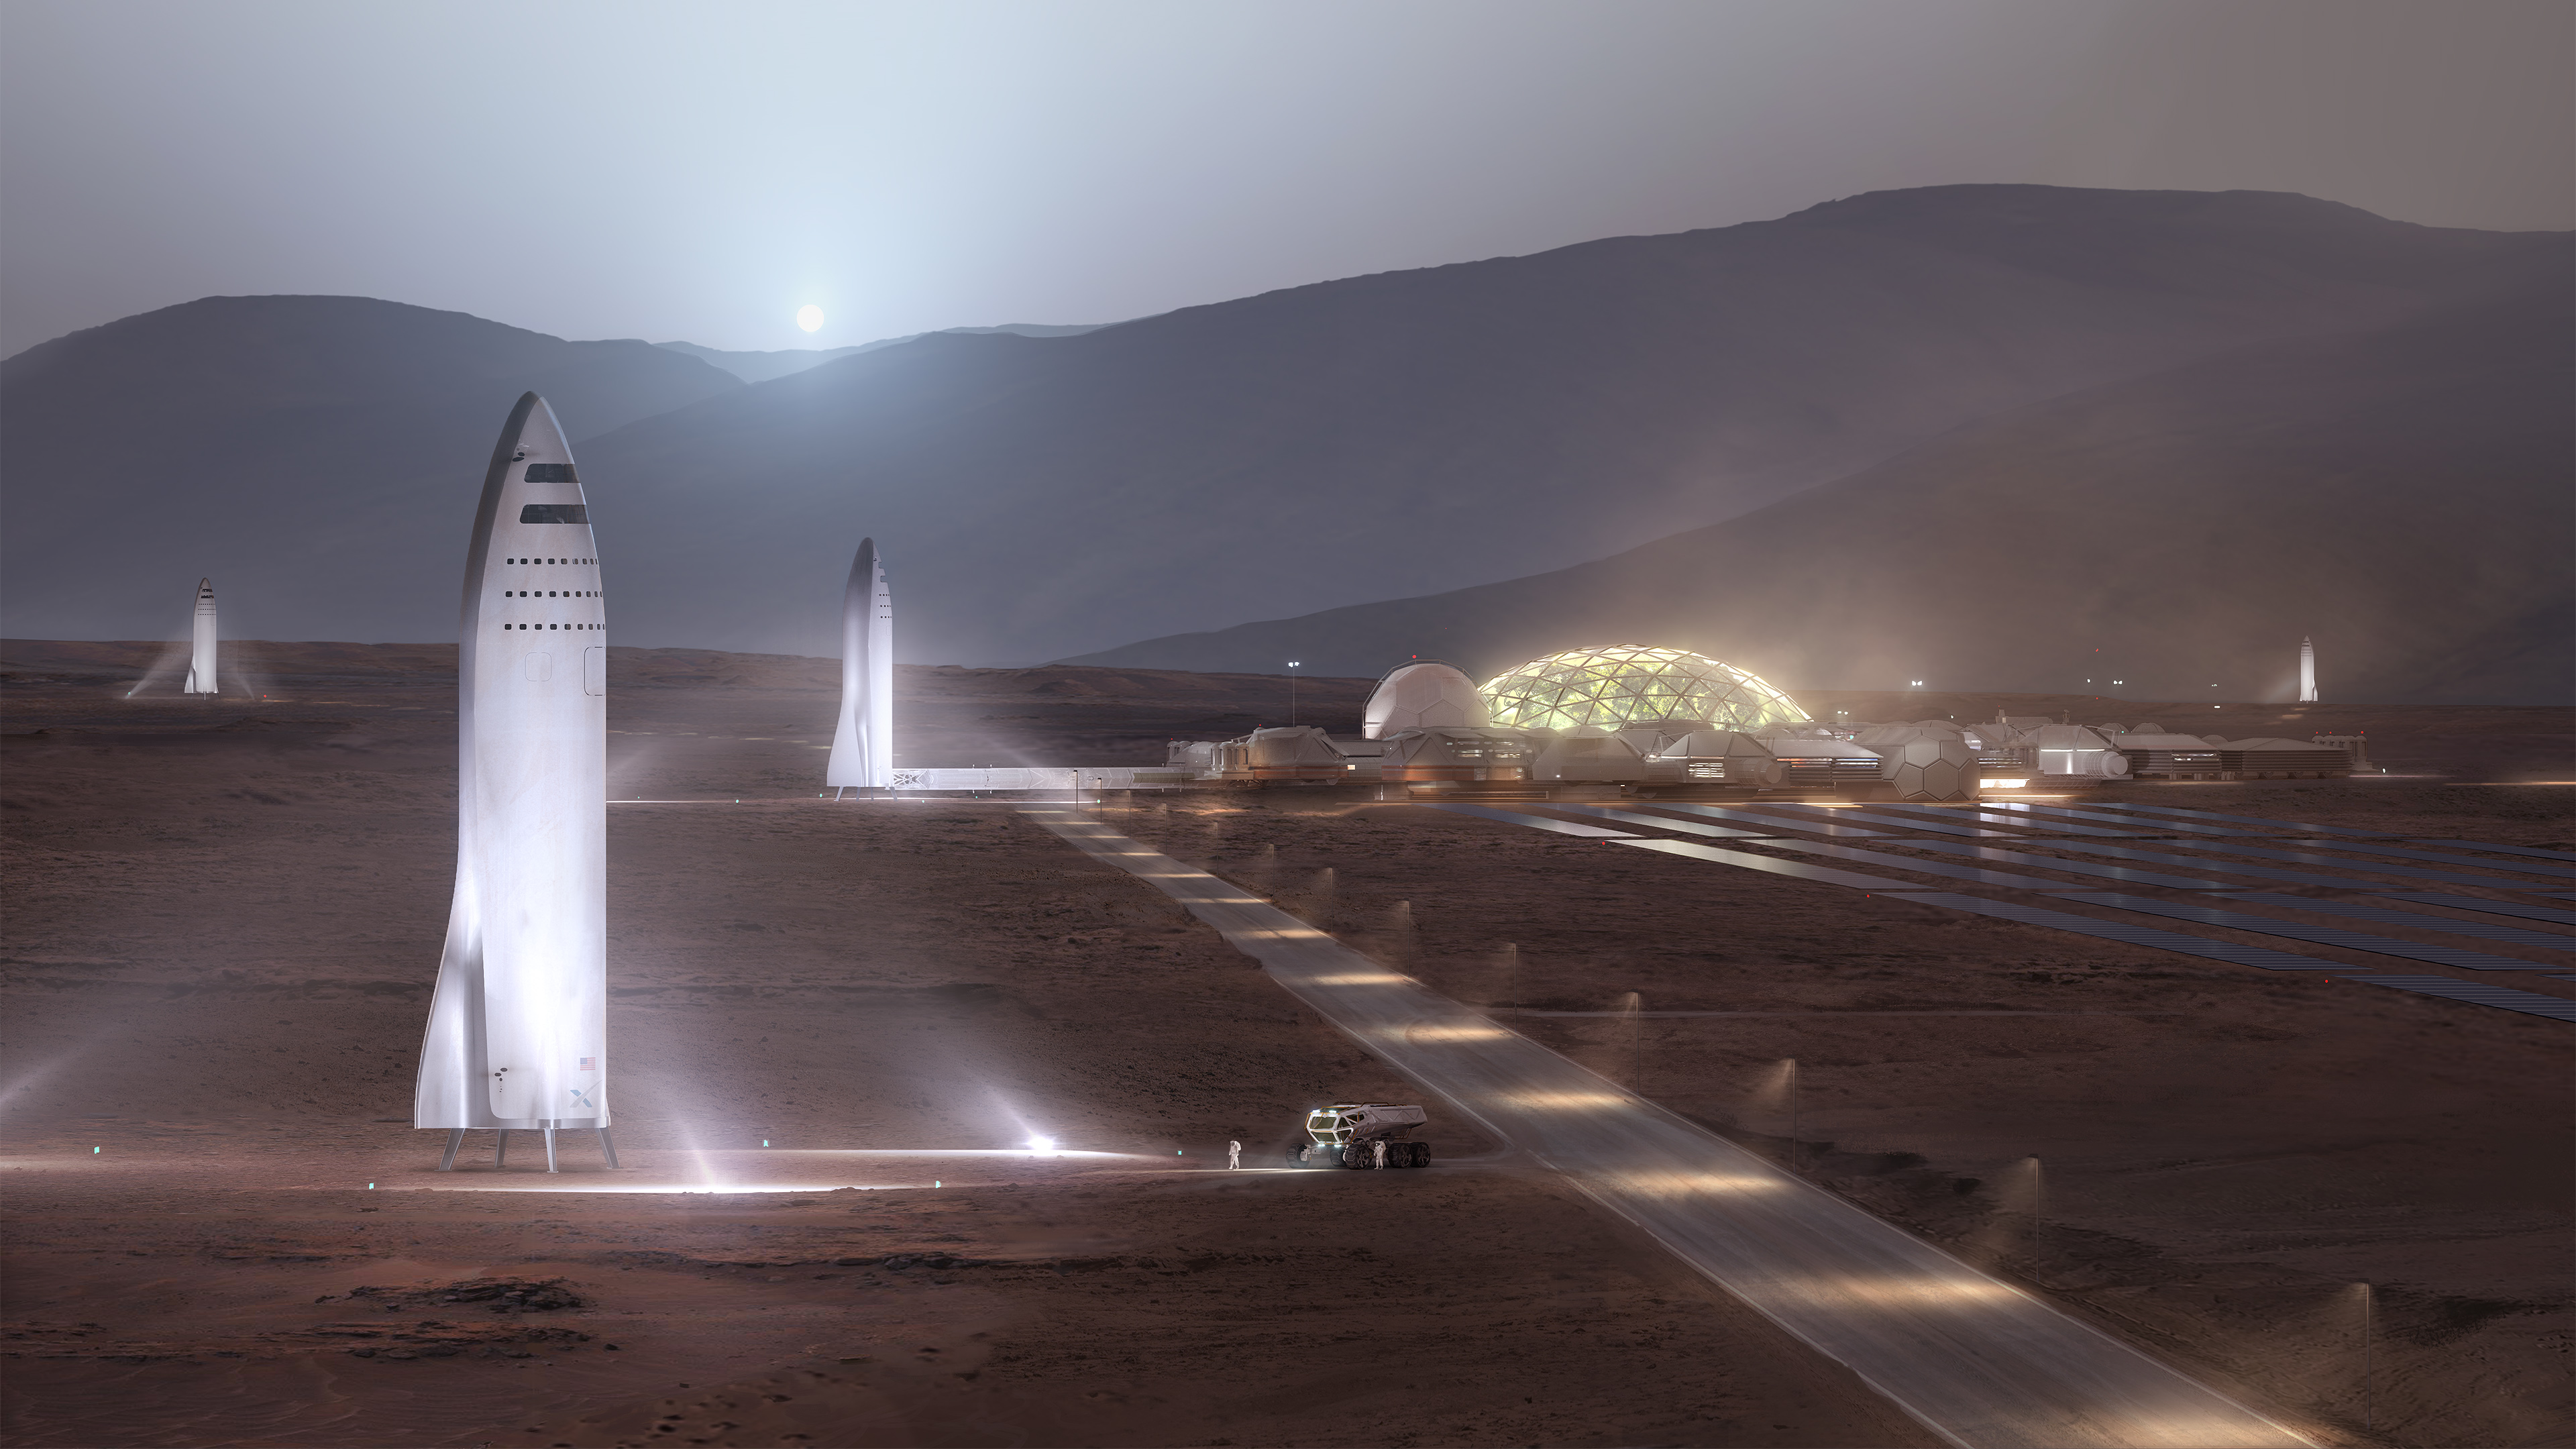
\includegraphics[width=\linewidth]{spacexmars}
			
			{\tiny Missions to Mars,
				\\ Quelle: spacex.com}}
		
		\only<2>{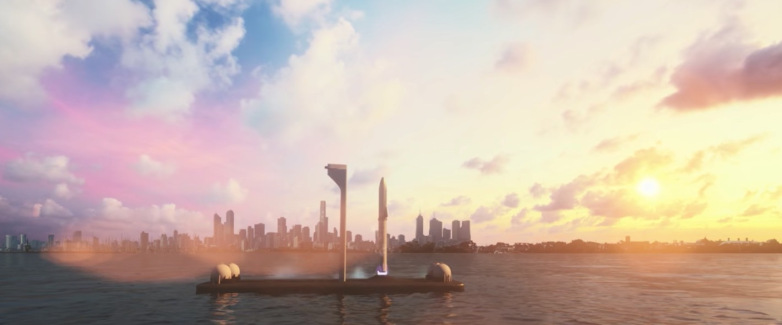
\includegraphics[width=\linewidth]{earthtoearth}
			
			{\tiny BFR: Earth to Earth,
				\\ Quelle: spacex.com}}
	\end{minipage}
\end{frame}

\subsection{CNSA}
\begin{frame}{\insertsection: \insertsubsection}
\begin{minipage}{.45\textwidth}
	
	2025 - 2060: \\
	\textbf{Space based solar power} \\
	
	\note<1>{
		\begin{itemize}
			\item China hat 2050 ein Energiedefizit von 10\%
			\item 55\% - 65\% des Sonnenlichts werden in der Atmosphäre in Wärme umgewandelt
			\item Umwandlung in Mikrowellen vermeidet das Problem
		\end{itemize}
	}

	
\end{minipage} \quad
\begin{minipage}{.5\textwidth}	
	
\includegraphics[width=\linewidth]{cnsa}
		
	{\tiny CNSA Logo,
		\\ Quelle: space.com}
\end{minipage}
\end{frame}
\subsection{Satelliten-Entwicklung}
\begin{frame}{\insertsection: \insertsubsection}
	\begin{minipage}{.45\textwidth}
		
		\textbf{GNSS}
		\vspace{12pt}
		\only<1,2>{
		\begin{itemize}
			\item GPS \& GLONASS
			\item Galileo \& Beidou
		\end{itemize}
		}
		\vspace{12pt}
		\pause
		\pause
		\textbf{\\Erdbeobachtung}
		\vspace{12pt}
		\only<4,3>{
		\begin{itemize}
			\item Terrain Kartierung
		
			\item Optische Beobachtung
		\end{itemize}
		}
		\vspace{12pt}
		\pause
		\pause
		\textbf{\\Andere Satelliten}
		\vspace{12pt}
		\only<4>{
		\begin{itemize}
			\item Satelliten-Internet
			\item Fernsehen etc.
		\end{itemize}
		}
		
		
		\note<1>{
			GPS GLONASS		
			\begin{itemize}
				\item GNSS Begriff (Global Navigational Satellite System)
				\item GLONASS Entwicklung (GNSS auf Russisch)
				\item GPS neue Daten (Global Positioning System)
				\item Galileo praktisch einsatzbereit
				\item bis 2020 online mit 30 Satelliten
				\item Beidou seit 2012 lokal China
				\item Bis 2020 35 Satelliten
			\end{itemize}
		}
		\note<2>{
			Galileo Beidou	
			\begin{itemize}
				\item Galileo praktisch einsatzbereit
				\item bis 2020 online mit 30 Satelliten
				\item Beidou seit 2012 lokal China
				\item Bis 2020 35 Satelliten
			\end{itemize}
		}
		\note<3>{
			Terrain		
			\begin{itemize}
				\item genaue Vermessung der Erde mit hoher Auflösung
				\item Navigation, Geologie und Katastrophenschutz
			\end{itemize}
		}
		\note<4>{
			Optisch		
			\begin{itemize}
				\item Hochauflösende Kameras
				\item Interpolation aktueller Entwicklungen zeigen starke Verbesserung
			\end{itemize}
		}
		\note<5>{
			Andere		
			\begin{itemize}
				\item Internet und Telephon über Satellit eher Nische
				\item mit besserer Technologie eventuell massentauglich
				\item Fernsehen etc nur technische Verbesserungen
			\end{itemize}
		}
	
	\end{minipage} \quad
	\begin{minipage}{.5\textwidth}
	\begin{center}
		\only<1>{
		
\includegraphics[width=.95\linewidth]{gps}}
		\only<2>{
		
\includegraphics[width=.95\linewidth]{galileo}}
		\only<3>{
		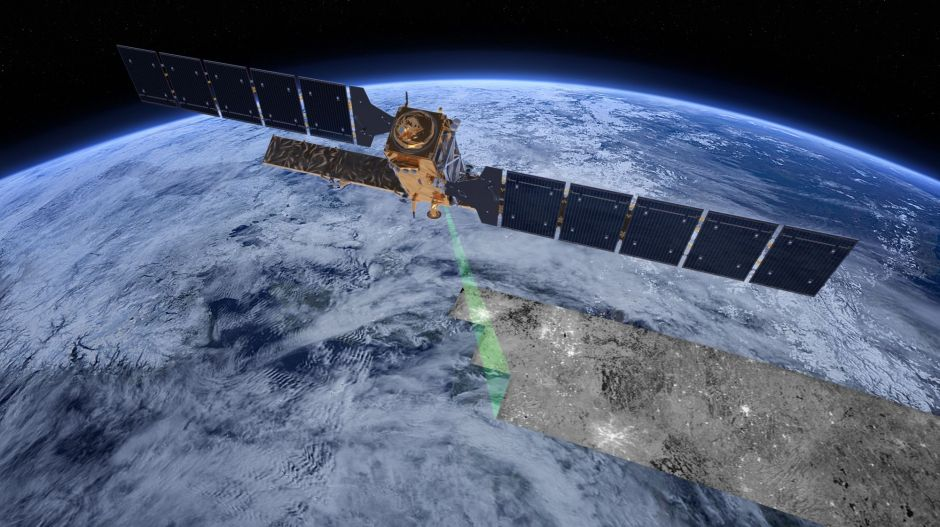
\includegraphics[width=.95\linewidth]{erdbeobachter}}
		\only<4>{
		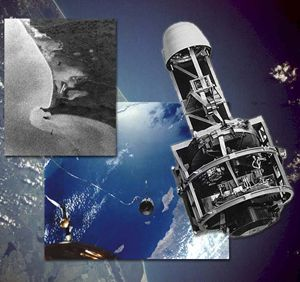
\includegraphics[width=.95\linewidth]{spionage}}
		\only<5>{
		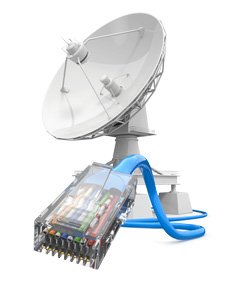
\includegraphics[width=.95\linewidth]{internet}}
	\end{center}	
	
	\only<1>{\tiny GPS Logo
		\\ Quelle: wikipedia.org}
	\only<1>{\tiny Galileo Logo
		\\ Quelle: wikipedia.org}
	\only<3>{\tiny Erdbeobachtungssatellit Sentinel
		\\ Quelle: wikipedia.org}
	\only<4>{\tiny Spionagesatellit Keyhole
		\\ Quelle: wikipedia.org}
	\only<5>{\tiny Satelliten-Internet
		\\ Quelle: wieistmeineip.de}
	\end{minipage}
\end{frame}
\section{Ferne Zukunft}
\subsection{Antriebe der Zukunft}
	
\begin{frame}{\insertsection: \insertsubsection}
	\begin{minipage}{.45\textwidth}	
		\textbf{Electro Dynamic Tethering}
		
		\vspace{12pt}
		
		\note<1>{
			Ort			
			\begin{itemize}
				\item Tether: Leine
				\item Nutzt Energie und Erdmagnetfeld als Antrieb
				\item Sehr Effizient
				\item Wenig Schub
			\end{itemize}
		}
	
		\pause
		
		\textbf{Ionen Antrieb}
		
		\note<2>{
			Größe
			\begin{itemize}
				\item Hall-Effect-Thrusters (HET): Nutzt Magnet um Xenon-Ionen zu beschleunigen, Ionisierung durch Anode
				\item Variable Specific Impulse Magnetoplasma Rocket (VASIMR): Nutzt Radiowellen zum ionisieren und erhitzen
			\end{itemize}
		}
		
	\end{minipage} \quad
	\begin{minipage}{.5\textwidth}	
		\only<1>{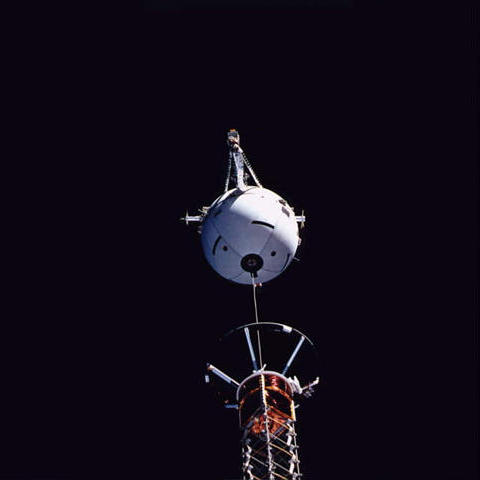
\includegraphics[width=\linewidth]{spacetether}
		
		{\tiny STS-75 Onboard View,
			\\ Quelle: nasa.gov}}
		
		\only<2>{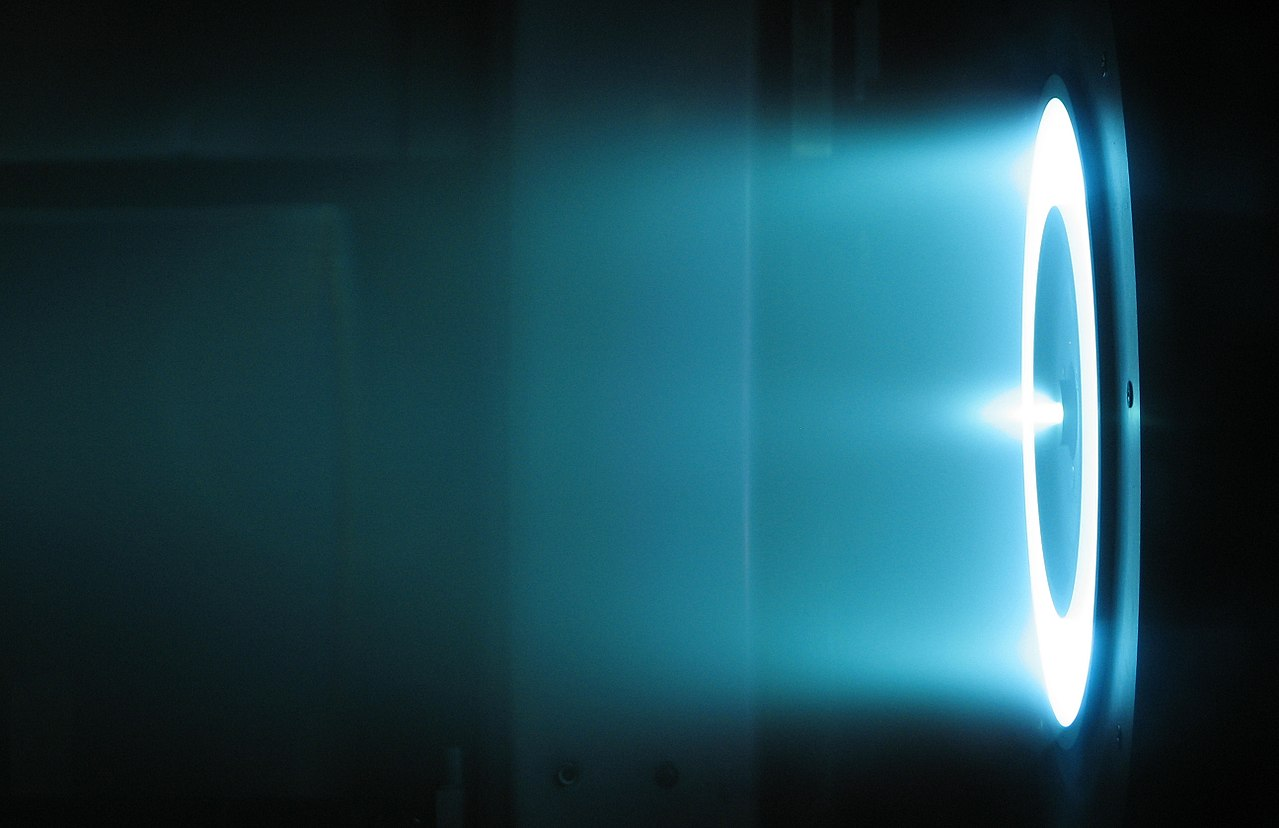
\includegraphics[width=\linewidth]{ionengine}
			
		{\tiny 6 kW Hall thruster,
			\\ Quelle: jpt.nasa.gov}}
	\end{minipage}
\end{frame}
%\begin{frame}{\insertsection: \insertsubsection}
%	\begin{minipage}{.45\textwidth}
%		
%		\textbf{Vergleich: Spezifischer Impuls}
%		\only<1>{
%			\begin{equation*}
%			\Delta v = v_{exh} \cdot \ln\left(\frac{M_0}{M_1}\right)
%			\end{equation*}
%		}
%		
%		\vspace{12pt}
%		
%		\note<1>{
%			Spezifischer Impuls			
%			\begin{itemize}
%				\item Abgasgeschwindigkeit
%				\item Maß für Effizienz eines Antriebs
%			\end{itemize}
%		}
%	
%	\end{minipage} \quad
%	\begin{minipage}{.5\textwidth}
%	\begin{center}
%		\includegraphics[width=.7\linewidth]{mainengine}
%	\end{center}	
%	
%	{\tiny Space Shuttle Main Engine
%		\\ Quelle: nasa.gov}
%	\end{minipage}
%\end{frame}
\subsection{Faster than Light Antriebe}
\begin{frame}{\insertsection: \insertsubsection}
	\begin{minipage}{.45\textwidth}
		
		\textbf{Warp Antrieb}
		\vspace{12pt}
		\only<1,2>{
		\begin{itemize}
			\item Herkunft
			\item Idee
		\end{itemize}
		}
		\pause
		\pause
		\vspace{12pt}
		\textbf{\\Wurmloch Generator}
		\vspace{12pt}
		\only<3,4>{
		\begin{itemize}
			\item Herkunft
			\item Idee
		\end{itemize}
		}
		\pause
		\pause
		\vspace{12pt}
		\textbf{\\Andere Möglichkeiten}
		\vspace{12pt}
		\only<5>{
		\begin{itemize}
			\item Weltraum Routen
			\item Generationen-Schiffe
		\end{itemize}
		}
		
		
		\note<1,2>{
			Warp Antrieb		
			\begin{itemize}
				\item Bedeutet "Verzerrung" der Raumzeit
				\item Erste Erwähnung  bei Star Treck
				\item Erste Idee "Flight of a Starling 1945 (von Chester S. Geier)
				\item Verschiebt Raumzeit um Weg zu verkürzen
				\item Nicht unbedingt entgegen Relativitätstheorie
			\end{itemize}
		}
		\note<3,4>{
			Wurmloch Generator		
			\begin{itemize}
				\item Öffnet eine Art Portal zu einer anderen Stelle des Universums.
				\item Begriff "Wurmloch" geprägt von John Wheeler.
				\item Bekannt durch die Serien "Stargate" und "Deep Space Nine".
				\item Ermöglicht eine instantane Reise zum Ziel.
				\item Widerspricht aktuellem Wissenschaftlichen Kenntnisstand.
			\end{itemize}
		}
		\note<5>{
			Alternativen		
			\begin{itemize}
				\item Weltraum Routen: Englisch Hyper-Lanes
				\item Ermöglichen Fortbewegung auf fest definierten Routen
				\item wenig Erklärung oder Erklärung über Warp-Antrieb
				\item Generationen-Schiffe: Nicht wirklich FTL
			\end{itemize}
		}
	
	\end{minipage} \quad
	\begin{minipage}{.5\textwidth}
	\begin{center}
		\only<1>{
		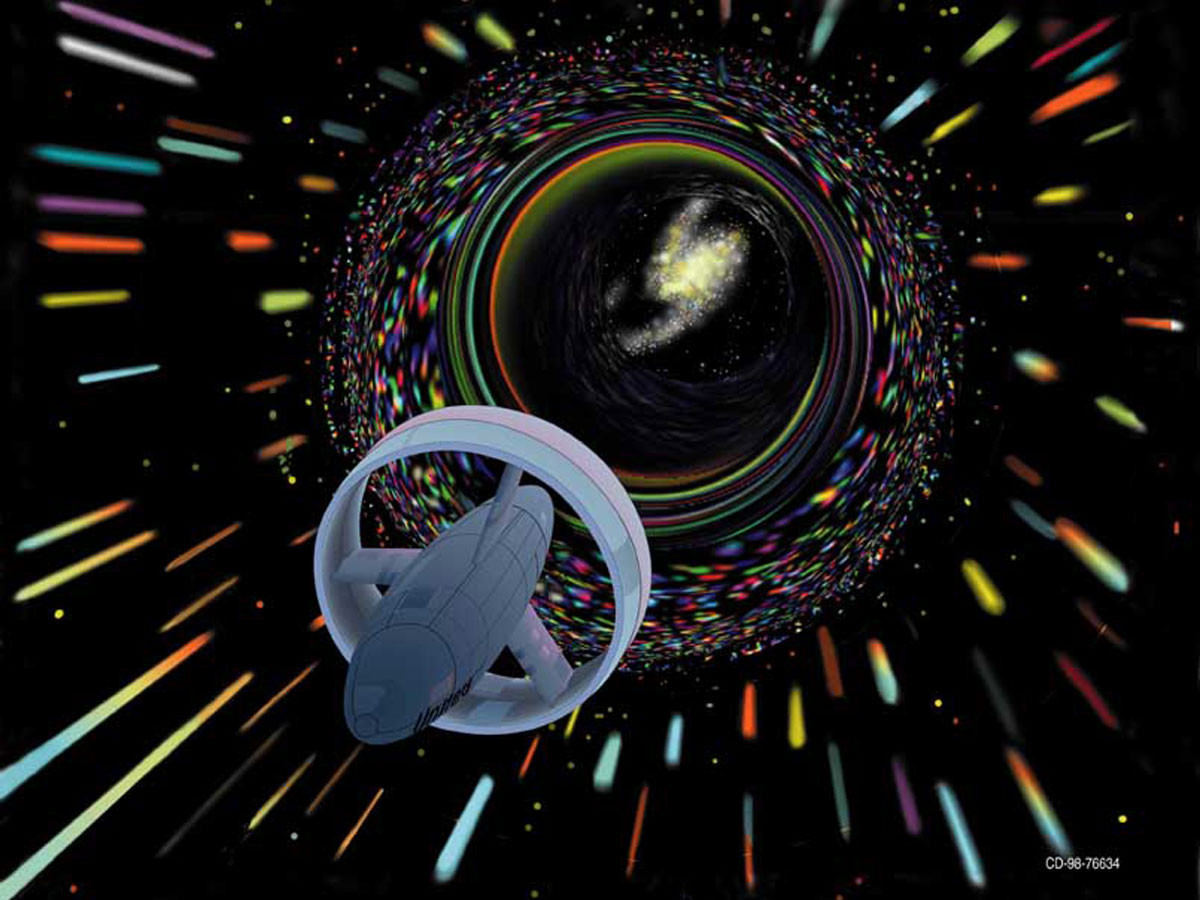
\includegraphics[width=.95\linewidth]{Warpantrieb}}
		\only<2>{
		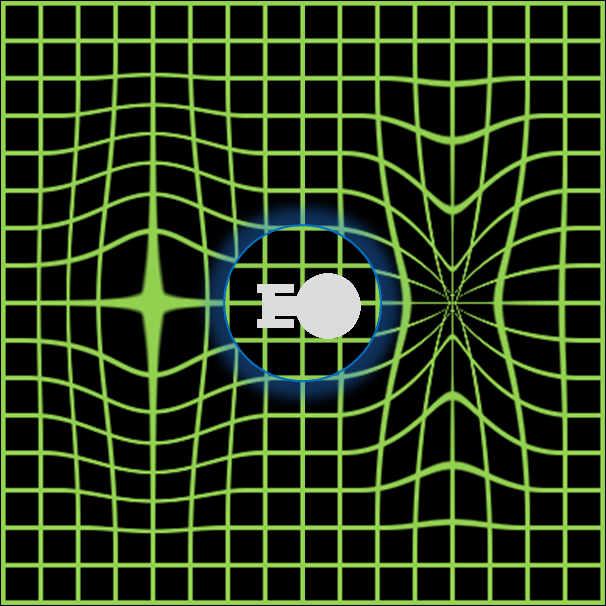
\includegraphics[width=.95\linewidth]{Warpfield}}
		\only<3>{
		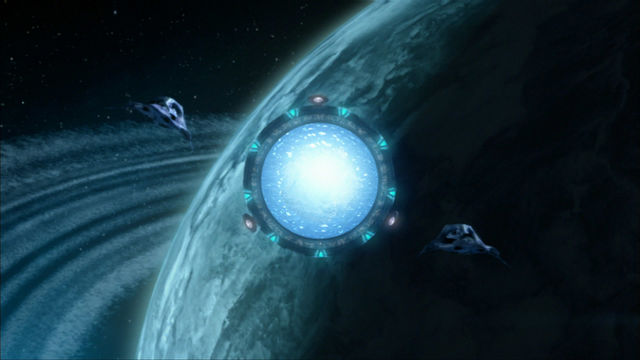
\includegraphics[width=.95\linewidth]{Stargate}}
		\only<4>{
		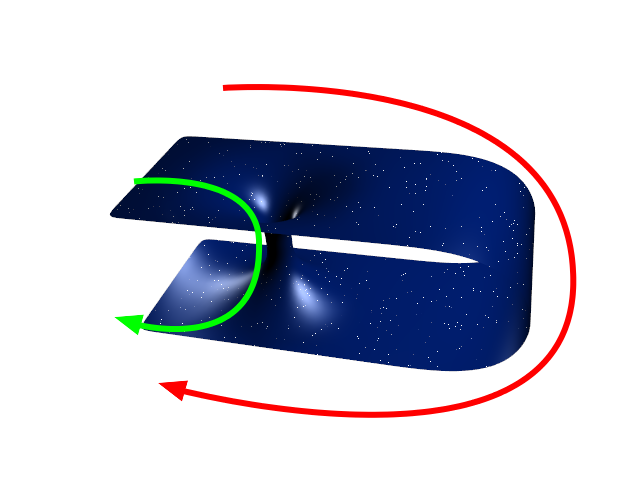
\includegraphics[width=.95\linewidth]{Wormhole}}
		\only<5>{
		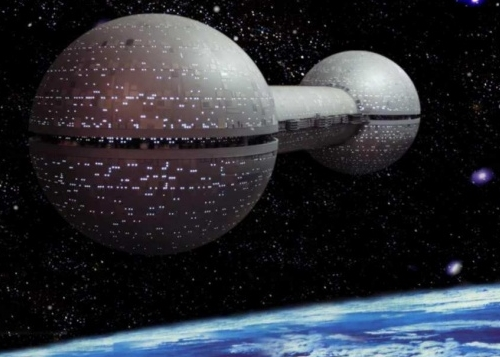
\includegraphics[width=.95\linewidth]{generationenschiff}}
	\end{center}	
	
	\only<1>{\tiny Übergang zu Warpgeschwindigkeit
		\\ Quelle: wikipedia.org}
	\only<2>{\tiny Funktion des Warp-Feldes bei Star Treck
		\\ Quelle: wikipedia.org}
	\only<3>{\tiny Wurmlochgenerator
		\\ Quelle: stargate.wikia.com}
	\only<4>{\tiny Funktion eines Wurmlochs
		\\ Quelle: wikipedia.org}
	\only<4>{\tiny Generationen-Schiff
		\\ Quelle: phoxim.de}
	\end{minipage}
\end{frame}
\subsection{Weltraumkolonien}
\begin{frame}{\insertsection: \insertsubsection}
\begin{minipage}{.45\textwidth}
	
	\textbf{Ursache}
	\only<1>{
	\begin{itemize}
		\item Religion
		\item Geld
		\item Ressourcen
	\end{itemize}
	}

	\vspace{12pt}
	
	\note<1>{
		Ursache			
		\begin{itemize}
			\item Religion
			\item Geld
			\item Ressourcen (Platz, Rohstoffe)
		\end{itemize}
	}

	\textbf{Ort}
	\only<2>{
		\begin{itemize}
			\item Planet
			\item Asteroid
			\item Struktur
		\end{itemize}
	}

	\vspace{12pt}
	
	\note<2>{
		Ort			
		\begin{itemize}
			\item Planet
			\item Asteroid (kann sogar verlegt werden)
			\item Selbstgebaute Struktur (z.B. Todesstern aus Star Wars, auch nur vorrübergehend vgl. Interstellar)
		\end{itemize}
	}

	\textbf{Größe}
	
	\note<3>{
		Größe
		\begin{itemize}
			\item Abhängig von Entfernung zur Erde bzw. zur nächsten großen Kolonie
			\item Bestimmtes Grundpersonal muss vorhanden sein: Medizin, Feuerwehr, Polizei, Anwälte, Richter, Verwaltungsapparat
			\item Erdnah (schnelle Kommunikation): mind. 100 Menschen, erdfern mind 1000 Menschen
		\end{itemize}
	}
	
\end{minipage} \quad
\begin{minipage}{.5\textwidth}	
	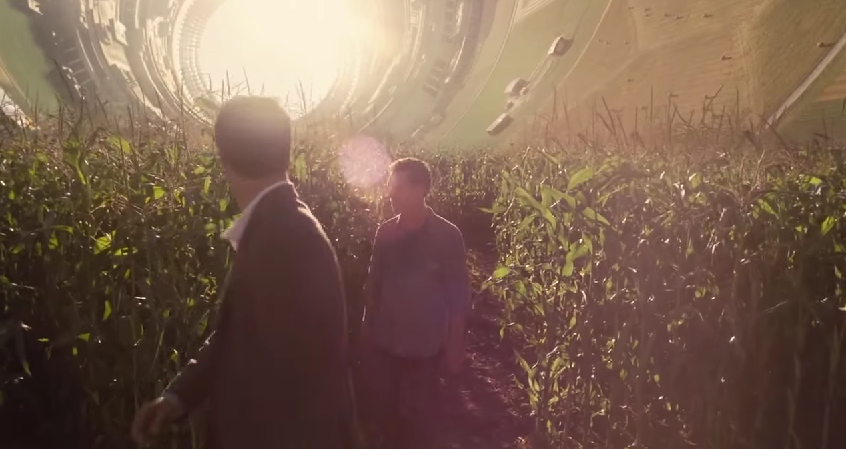
\includegraphics[width=\linewidth]{cooper_station}
	
	{\tiny "Cooper Station",
		\\ Quelle: Interstellar, Warner Bros. Pictures}
\end{minipage}
\end{frame}

\end{document}
